\subsubsection{{Математическая библиотека}}
\addcontentsline{toc}{subsubsection}

Математическая библиотека занимает главенствующую роль в проекте, так как именно она содержит
набор алгоритмов, позволяющих получить генеральный план площадного объекта в автоматическом режиме.

Прежде чем изобразить архитектуру математической библиотеки, сформулируем основные концепции,
которые будут её описывать.
Для исследовательских проектов именно общие принципы реализации
приобретают главенствующую роль, так как в силу очень высокой динамичности изменений требований к результату работы
и несистемности этих требований отсутствует какая-либо возможность спроектировать архитектуру заранее.

\textit{Математическая методика} является классом алгоритмов, которые могут решать ту или иную задачу.
Каждая математическая методика используется хотя бы в одном \textit{математическом методе}.

\begin{itemize}
    \item {
        \textit{Аккуратное использование внешних зависимостей.}
        Исходный код математической библиотеки является главным результатом работы команды исследователей,
        поэтому, по-возможности, он должен содержать наименьшее количество внешних зависимостей.
        Допускается использование математических и научных библиотек языка Python.
    }
    \item {
        \textit{Каждая математическая методика должна быть выделена в отдельный программный модуль.}
        Так как каждая методика олицетворяет собой определенный класс математических алгоритмов,
        а сами алгоритмы являются концептуально сложными, то для упрощения их поддержки и модернизации
        следует ввести их явное логическое разделение.
    }
    \item {
        \textit{Минимализм во входных и выходных данных каждой методики.}
        В рамках каждой методики должны использоваться только лишь те данные, которые необходимы для её работы.
        Использования лишних данных следует избегать.
        Данная концепция обусловлена тем, что в силу высокой сложности алгоритмов,
        очень важно уменьшать накладные расходы на их отладку, что может сильно осложняться
        из-за большого количества входных параметров.
    }
    \item {
        \textit{Все параметры каждой методики должны быть выделены в отдельный класс.}
        Внутри реализации каждой математической методики недопустимо появление различных "магических чисел".
        Применение этой концепции обусловлено необходимостью повторяемости научного эксперимента.
        Если спрятать параметры алгоритма внутрь исходного кода, то результат на одних и тех же исходных данных
        может неудастся повторить в силу потерянного значения одного из чисел.
    }
    \item {
        \textit{Входные/выходные данные и параметры каждой методики должны быть сериализуемыми.}
        Так как расчёты могут производиться, как на сервере, так и на компьютере исследователя, то необходимо
        предусмотреть механизм простой передачи данных с компьютера на сервер и обратно. Самым простым способом
        является сериализация входных и выходных данных.
    }
\end{itemize}

Ниже представлена верхнеуровневая диаграмма классов математического
модуля(см. рисунок \ \ref{pic:architecture__math-classes}).

\begin{figure}[H]
	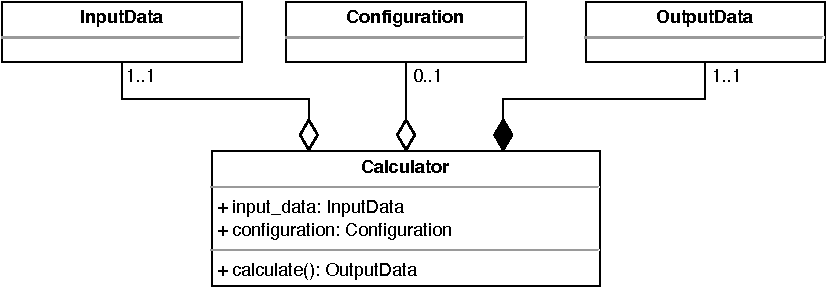
\includegraphics[width=0.6\textwidth, left]{architecture/pictures/math/classes}
	\caption{Верхнеуровневая диаграмма классов математического модуля}
	\label{pic:architecture__math-classes}
\end{figure}
\vskip 5 mm

Каждая алгоритмическая методика запускается путём вызова метода \textit{calculate}
в классе \textit{Calculator}.
Для каждой методики может быть реализовано несколько интерфейсов \textit{Calculator},
которые будут использовать один класс алгоритмов, но давать несколько иной результат.

Каждая реализация \textit{Calculator} принимает входные данные \textit{InputData}
и возвращает выходные данные \textit{OutputData}.
Если методика подразумевает использование различных параметров настройки, то \textit{Calculator} дополнительно
принимает на вход \textit{Configuration}. Если параметры настройки не требуются, то класс \textit{Configuration}
является \textit{NULL}.
